%01/10 
\chapter{Segmentación de imágenes}
\section{Introducción}
La segmentación de imágenes tiene como objetivo la partición de una imagen en regiones o segmentos homogéneos con respecto a alguna característica (color, forma, distancia, tamaño) con el fin de simplificarla e identificar elementos de interés para una aplicación concreta. Toda la imagen está segmentada y la unión de los fragmentos recupera por completo la imagen.

En medicina, las aplicaciones de la segmentación incluyen la detección del borde coronario en angiogramas, medición del volumen tumoral y su respuesta a la terapia, mapeo funcional, clasificación automatizada de células sanguíneas, detección de microcalcificaciones en mamografías, extracción de imágenes del corazón a partir de cineangiogramas cardíacos, detección de tumores, etc.

La región $\Omega_j$ se define por un conjunto de píxeles "similares" de acuerdo a alguna característica definida sobre los píxeles de la imagen. 

Al medir la luminancia y conectividad, se miden si los píxeles se tocan (son conexos) o no (están segmentados). En una conectividad de 4, los píxeles que son conexos son los de arriba y abajo con respecto al píxel en cuestión, mientras que una conectividad de 8 implica que todos los de alrededor (incluidos los de la diagonal) son conexos. La luminancia y conectividad nos permiten diferenciar correctamente.

\begin{figure}[h]
\centering
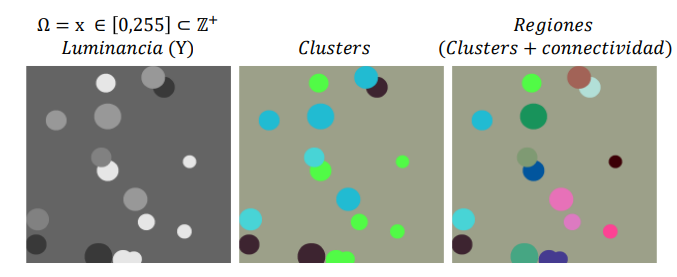
\includegraphics[width = 0.8\textwidth]{figs/luminancia-conectividad.png}
\end{figure}

Se utiliza una \textbf{etiqueta o label} como identificador de la región en la segmentación. Puede tener un número o color aleatorio y simplemente indica las regiones independientes y por tanto diferentes a las demás. 

Un \textbf{representante} es un descriptor de las características de la región de igual dimensión (d) que el espacio de decisión. Se realiza la estadística de lo que se quiere representar (media, mediana, moda). 

El \textbf{contorno} se define como el conjunto de píxeles alrededor de la región $\Omega_j$ en cuyo vecindario 9 hay al menos un píxel perteneciente a la región $j$ y un píxel no perteneciente a la región $j$. 

Sin embargo, esto está mal condicionado, ya que no hay un criterio para definir una región. Diferentes usuarios pueden considerar diferentes regiones y diferentes anotaciones. Además, el resultado depende de la escala y el conocimiento previo que se pueda tener ayuda a tomar las decisiones.

Hay distintos tipos de segmentación:
\begin{itemize}
\item \textbf{Clases:} separar objetos de su entorno, como por ejemplo separar una vaca del fondo de la imagen.
\item \textbf{Instancias:} separar  objetos individuales, para poder diferenciar por ejemplo dos personas juntas del fondo y entre ellas.
\item \textbf{Partes:} se identifican las distintas partes de los objetos
\item \textbf{Partes (alto nivel):} se siguen identificando las distintas partes de los objetos, pero sin tanto detalle, siendo así un punto intermedio entre instancias y partes.
\end{itemize}

\section{Técnicas más representativas}
Las técnicas más representativas se pueden clasificar en manual, semiautomáticas o automáticas, si son segmentación a bajo nivel o basada en modelo, o si son clásicas, basadas en estadísticos, difusas o redes convolucionales.

\subsection{Umbralización (operador puntual}
La umbralización o \textit{thresholding} es un caso particular de recorte para $a = b = T$. Así, la primera y última pendiente son nulas y la intermedia es absoluta. El threshold es un binario que divide la imagen en dos regiones, siendo así muy útil para imágenes bimodales.

Es útil para eliminar niveles cuando se sabe que el original sólo tiene dos y, en general, en la toma de decisiones binarias, como por ejemplo para finalizar la separación de objetos en procesos de segmentación.

\paragraph{Umbralización de imágenes bimodales}
Se utiliza un algoritmo que itera y, cuando la diferencia obtenida entre el nuevo umbral y el anterior es menor que la unidad, se detiene.

\paragraph{Método de Otsu}
Realiza una búsqueda exhaustiva del umbral que minimiza la varianza intra-clase. Busca el punto medio, pero teniendo en cuenta las distribuciones (variabilidad), permitiendo identificar objetos. 

\begin{figure}[h]
\centering
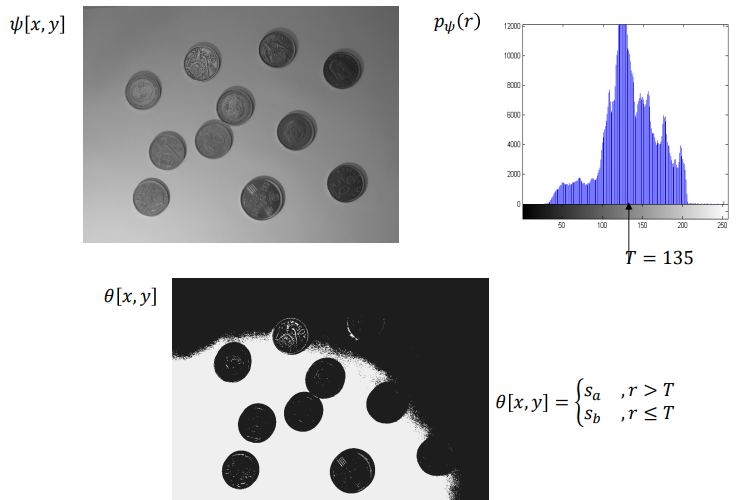
\includegraphics[width = 0.7\textwidth]{figs/umbralizacion-ej.png}
\caption{Si se utiliza la varianza para la umbralización, la imagen resultante (inferior) es muy mala al no realizar la separación entre fondo y monedas bien. Tanto la umbralización de imágenes bimodales como el método de Otsu son binomiales, y para este caso se debe segmentar en ventanas y aplicar la umbralización a cada ventana.}
\end{figure}

\begin{figure}[h]
\centering
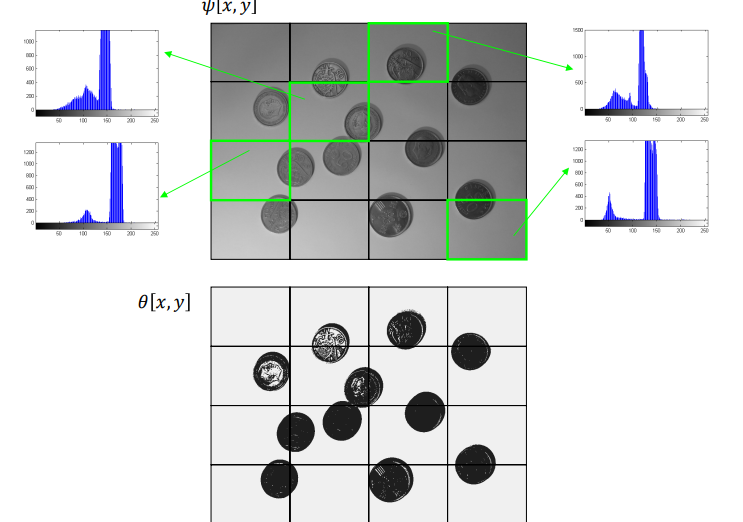
\includegraphics[width = 0.7\textwidth]{figs/umbralizacion-ej2.png}
\end{figure}

\paragraph{Multimodal} 
Para imágenes multimodales, se pueden aplicar los métodos anteriores bimodales repetidamente. De esta forma, primero se separan las dos regiones más grandes, y posteriormente de cada región se obtienen otras dos regiones contenidas en ella, etc. Esto se utiliza en la clasificación de tejidos mediante tomografía computarizada (CT). Mediante la consulta a expertos, se conoce la distribución y desviación de los tejidos. Estos datos se utilizan en algoritmos y se hacen medias dos a dos para poner un threshold.

\subsection{Clustering (agrupamiento por regiones)}
En el clustering, la imagen se divide entre K regiones más representativas. Las imágenes en color tienen un volumen de datos mayor, y el agrupamiento es díficil si se basa en el sistema visual humano.

Las aproximaciones son espacialmente "ciegas". La imagen se analiza como un conjunto de puntos d-dimensionales en el espacio de decisión. La técnica más representativa es \textbf{K-means}. Se busca la mejor frontera de separación entre los píxeles de sus vecinos más cercanos. 

Inicialmente hay tantos núcleos como píxeles. Cada núcleo tiene su celda, y se irán fusionando celdas si la distancia es menor que X. Esto se repite hasta obtener el número de clústeres que se quieran. El clustering clásico no tiene en cuenta el contorno, pero en imágnes RGB son 5 las variables que hay que tener en cuenta (rojo, verde, azul, x, y).
Los resultados dependen de la característica utilizada (feature space). Aunque nos regiones de la imagen sean del mismo color, se pueden segmentar en dos regiones utilizando similitud y proximidad.

El número de clústeres se escoge en función de lo que se busque ver.
\begin{figure}[h]
\centering
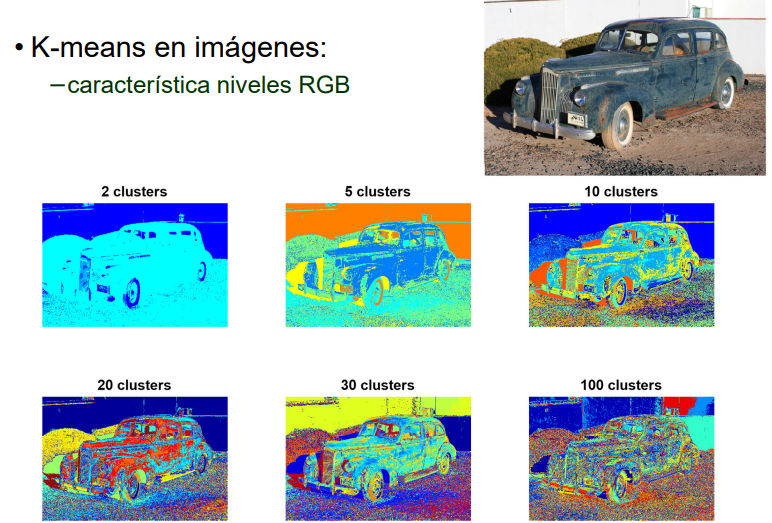
\includegraphics[width = 0.6\textwidth]{figs/clustering.png}
\end{figure}

\subsection{Detección y unión de bordes (basados en contornos)}
Se utiliza el detector de Canny, un algoritmo multietapa cuyo objetivo es localizar todos los bordes de una imagen con máxima precisión y sólo una vez cada borde. Las etapas se dividen en:
\begin{enumerate}
\item Suavizado de la imagen con un filtrado gaussiano. Esto sirve para que una imagen no se vea abrupta, sino continua.
\item Aproximación de la magnitud del gradiente y ángulo (Sobel/Prewitt).

Esto permite diferenciar los bordes en grados (ángulos de giro). Se hace la tangente y se calcula el ángulo. Saber el ángulo permite que, esté donde esté y tenga el grosor que tenga, se pueda obtener el punto medio analizando su perpendicular. 

\begin{figure}[h]
\centering
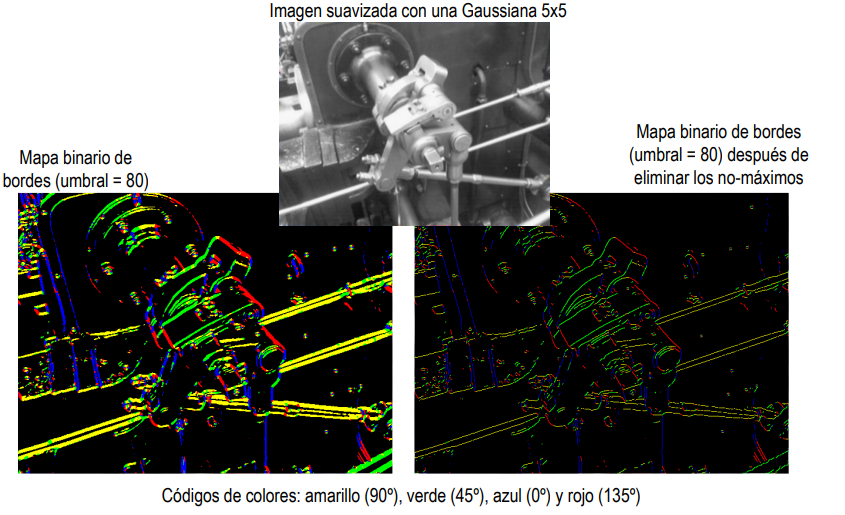
\includegraphics[width = 0.6\textwidth]{figs/deteccion-bordes.png}
\caption{La imagen izquierda tiene un grosor indefinido. La imagen derecha garantiza que todos tengan un borde de 1 píxel.}
\end{figure}

\item Umbralizado doble para detectar píxeles pertenecientes a bordes fuertes/débiles. Los bordes fuertes tienen grandes cambios de grises, mientras que los bordes suaves permiten cambios mínimos de grises.

\item Rechazo de píxeles en bordes débiles no conectados a bordes fuertes.
En el umbralizado alto, sólo se mantienen los bordes con cambios de gris muy exagerados de manera que hay granos de arroz que no terminan de asomarse.

\begin{figure}[h]
\centering
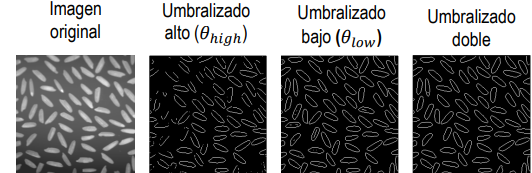
\includegraphics[width = 0.6\textwidth]{figs/bordes.png}
\end{figure} 
\end{enumerate}

\subsection{Contornos activos (basados en contornos)}
Los contornos activos snakes son un método global para la búsqueda de los contornos de los objetos en el espacio de decisión usando la imagen como soporte.

Es un proceso iterativo que busca rodear un objeto de interés, como puede ser un tumor. La snake se muestrea en un conjunto de puntos de control y busca minimizar una función de energía que combina:
\begin{itemize}
\item Energía interna: controla la deformación de la snake para evitar el sobreajuste.
\item Energía externa: controla el ajsute de la snake a los contornos para definir la calidad de la segmentación.
\item Energía restrictiva: restricciones de diseño, generalmente en función de la aplicación (ad hoc) o para incrementar la robustez al ruido.
\end{itemize}

El ajuste de snake se hace sobre una imagen de gradiente donde la curva tiende a meterse o salir del valle. Cuantas más iteraciones se hagan, mayor detalle se consigue.

\subsection{Redes convolucionales (deep learning)}
Las redes convolucionales (CNNs) son arquitecturas diseñadas para trabajar con datos estructurados espacialmente, como las imágenes médicas (microscopía, resonancia magnética, TAC, histología digital, etc.).

Un kernel (o filtro) es una pequeña matriz de pesos entrenables que se desplaza por la imagen (operación de convolución).
Cada kernel extrae un tipo de información: bordes, texturas, formas, o patrones más abstractos conforme se avanza en las capas.
Al principio, los kernels suelen detectar características de bajo nivel (bordes, contrastes), y en capas más profundas, rasgos de alto nivel (estructuras celulares, tejidos, órganos).

La idea es aplicar sucesivamente diferentes kernels entrenables de diferentes tamaños, diferentes niveles semánticos y combinar sucesivamente kernels a algunos más complejos.
Al aplicar convoluciones y pooling (submuestreo), la imagen va reduciendo su tamaño (se pierde resolución espacial). A cambio, las representaciones internas ganan en complejidad y profundidad: el número de canales (o mapas de características) aumenta. Esto genera un “código comprimido” de la imagen, útil para reconocer patrones globales.

\begin{figure}[h]
\centering
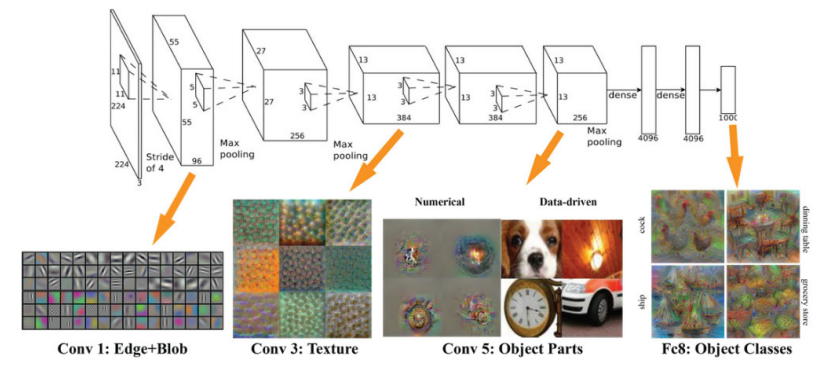
\includegraphics[width = 0.8\textwidth]{figs/convolutions.png}
\end{figure}

En clasificación, basta con decir si en la imagen hay un tumor o no. Pero en segmentación biomédica queremos una predicción a nivel de píxel (ej: qué píxeles son tumor, tejido sano, vasos sanguíneos, etc.). El \textbf{encoder} reduce la imagen extrayendo características relevantes. El \textbf{decoder} hace el proceso inverso, usando convoluciones transpuestas (deconvoluciones) o interpolaciones para recuperar la resolución original. Así, se obtiene un mapa de segmentación con la misma dimensión que la imagen inicial.

\begin{figure}[h]
\centering
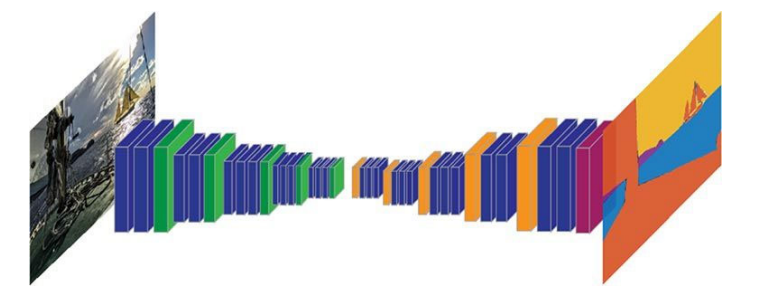
\includegraphics[width = 0.8\textwidth]{figs/encoder-decoder.png}
\end{figure}
